\begin{figure}[h!]
\begin{center}
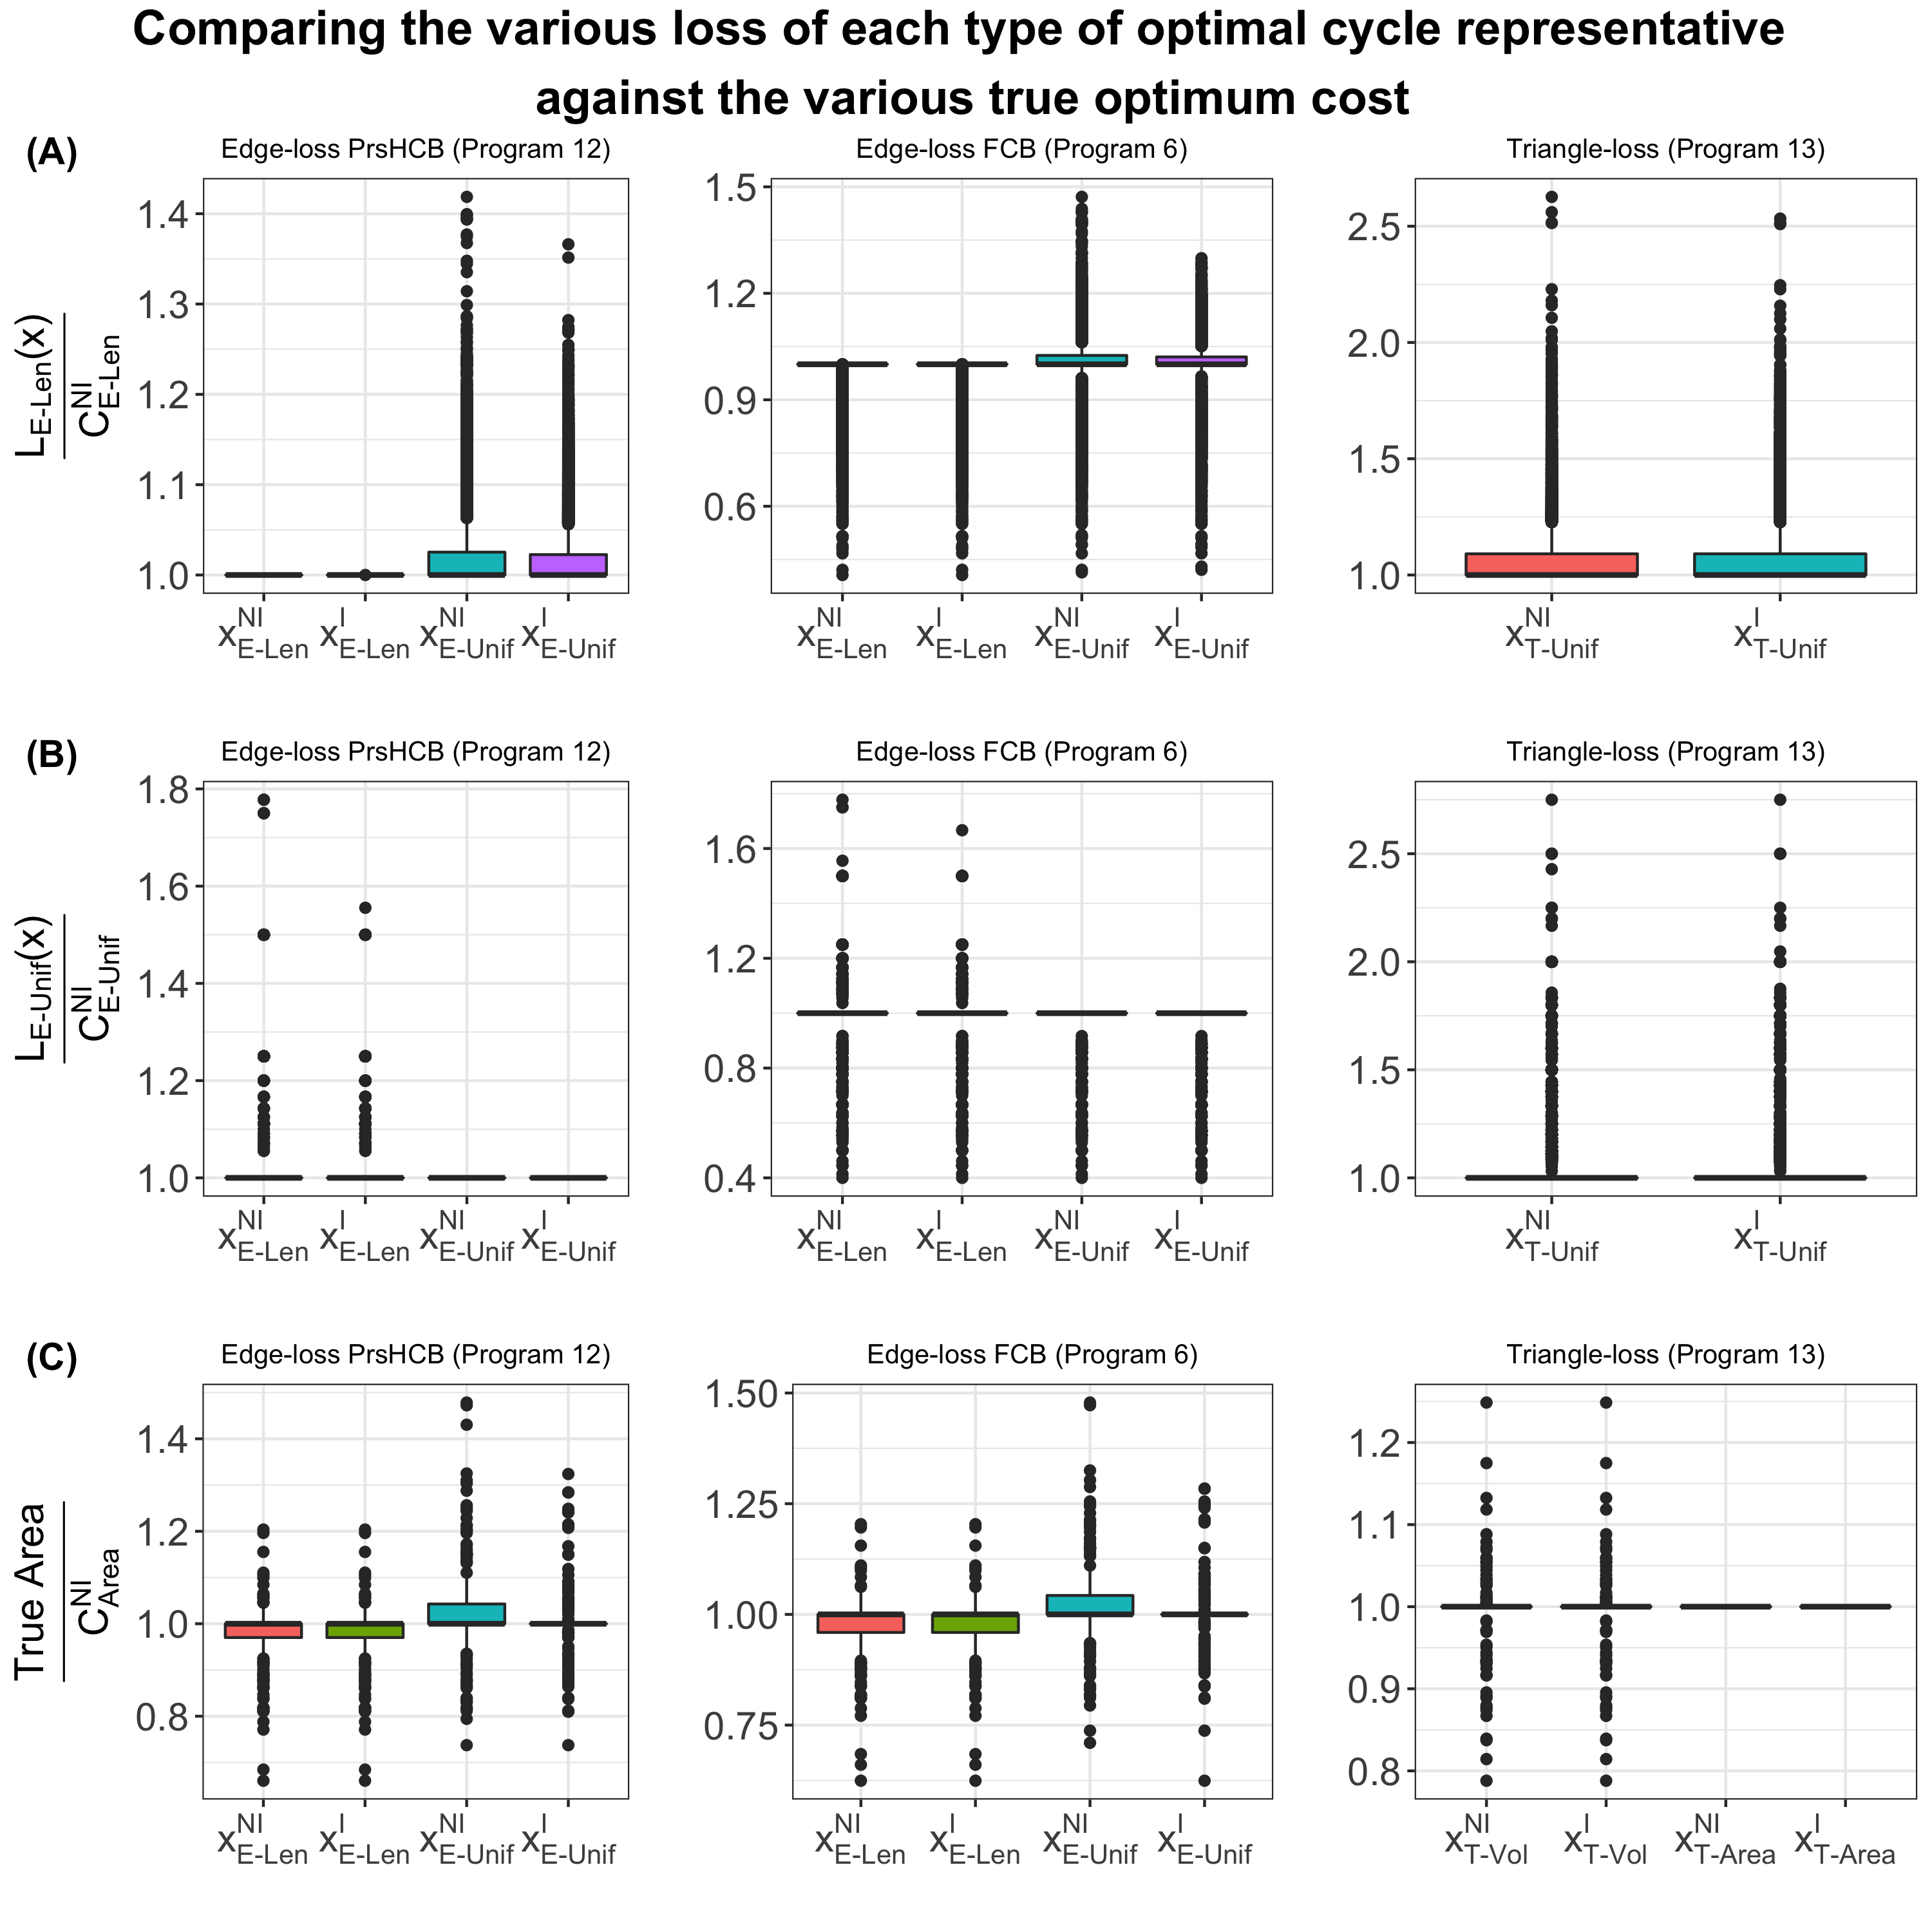
\includegraphics[width=\textwidth]{figures/length_area_edge.png}
\end{center}
\caption{Box plots of the ratios between (\textbf{A}) $L_{E\text{-}Len}(\optimalrep_\bullet^\bullet)$ and $C_{E\text{-}Len}$,  \textbf{(B)} $L_{E\text{-}Unif}(\optimalrep_\bullet^\bullet)$ and $C_{E\text{-}Unif}$, and  \textbf{(C)} $L_{T\text{-}Area}(\optimalrep_\bullet^\bullet)$ and $C_{T\text{-}Area}$. 
The horizontal axis is the type of optimal representative, $\optimalrep_\bullet^\bullet$, and the vertical axis is the ratio between the loss of each type of optimal representative over the actual cost of the optimal representative of the same loss function, i.e. the $\setofpersistenthcyclebases$ cycles which are solutions to Programs \ref{itm:edge_NIU}, \ref{itm:edge_NIL}, \ref{itm:tri_NIA}.
In \se \ref{coefficient}, we discussed that the optimum cost is the same whether we require an integer solution or not for essentially all solutions for \pr \eqref{eq:edgelossgeneral}, \pr \ref{eq:escolarargmin}, and the uniform-weighted triangle-loss method, resulting in two columns in the first two rows having ratio 1. The data used in \textbf{(A)} and \textbf{(B)} aggregate over all data described in \ref{sec: realworlddata} and \ref{sec: randompointclouds}. The data used in \textbf{(C)} aggregate the $190$ cycle representatives from $10$ point clouds from a normal distribution with ambient dimension of $2$. True area represents the total area enclosed by the representative, while $C_{Area}\NI$ represents the area of the area-weighted triangle-loss optimal cycle minimizing \ref{itm:tri_NIA}. We observe that some edge-loss optimal cycles and triangle-loss optimal cycles requiring integral solutions have an area smaller than that of the area-weighted triangle-loss optimal cycle. Refer to Figure \ref{fig:areaExample} and \se  \ref{sec:comparing optimal generators against different loss functions} to see why this may happen. 
% In addition to $\optimalrep_{Area}\NI = \optimalrep_{Area}\I$ for corresponding cycle representatives in all experiments, so too are $\optimalrep_{Len}\NI = \optimalrep_{Len}\I$.
}
 \label{fig:lengthcocmpare}
\end{figure}

